\documentclass{article}

\usepackage{amsmath}
\usepackage{geometry}
\usepackage[spanish]{babel}
\usepackage{graphicx}

\geometry{
    top=2cm,
    bottom=2cm,
    left=2cm,
    right=2cm
}

\title{Tarea 2 Metodos no Parametricos}
\author{Rudy Miranda}
\date{julio, 2023}

\begin{document}
    \maketitle 
    \tableofcontents

    \section{Introducci\'on}
    Se nos presenta el caso donde somos contratados por un instituto de estudio financieros para analizar los datos provenientes de 100 empresas del mercado bursatil y realizar comparaciones mediante disitintos test no parametricos.

    \section{Origen vs Tiempo}

    \begin{figure}[ht]
        \centering
        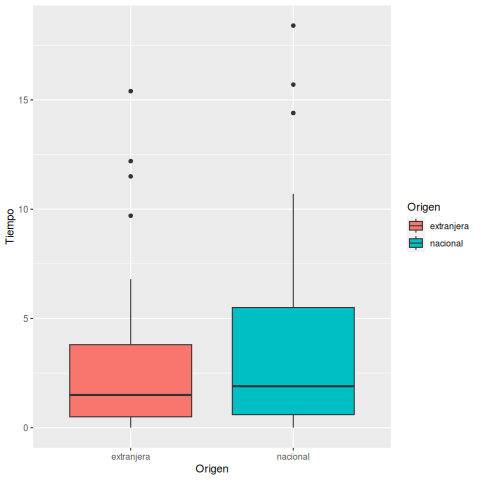
\includegraphics[width=0.7\linewidth]{../imgs/img1.png}
    \end{figure}

    mediante este boxplot podemos hacernos una idea de las caractisticas de los datos. Apoyaremos esto con un analisis descreptivo de los estad\'isticos mas comunes.
    
    \subsection{Analisis Descriptivo}

    \begin{figure}[ht]
        \centering
        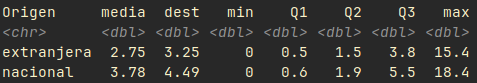
\includegraphics[scale=0.7]{../imgs/screenshot1.png}
    \end{figure}

    \newpage

    \section{Tipo vs Capitalizaci\'on}

    \begin{figure}[ht]
        \centering
        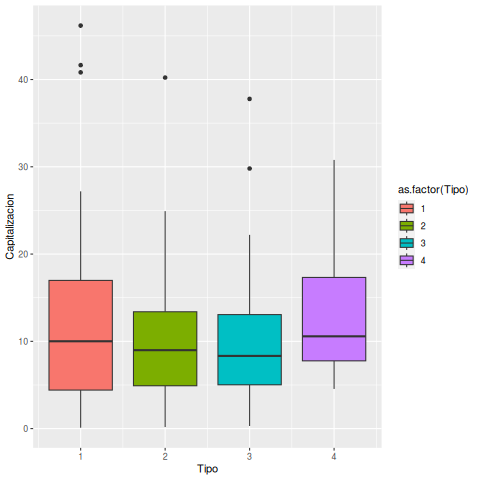
\includegraphics[width=0.7\textwidth]{../imgs/img2.png}
    \end{figure}
    
    \subsection{Analisis Descriptivo}

    \begin{figure}[ht]
        \centering
        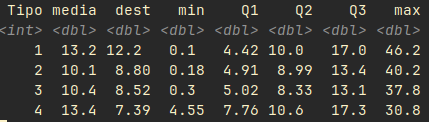
\includegraphics[width=0.7\textwidth]{../imgs/screenshot2.png}
    \end{figure}

    \section{Test de Mann-Whitney}
    \subsection{Hip\'otesis}
    \begin{equation}
        H_0:P(X_\text{Nacional} > X_\text{Extranjera}) = P(X_\text{Nacional} < X_\text{Extranjera})
    \end{equation}
    \begin{equation}
        H1: \text{no ocurre } H_0
    \end{equation}
    \subsection{Estad\'istico de Prueba y desarrollo del test}
    El estad\'istico de prueba para este caso es:
    \begin{equation}
        U = \min {U_1, U_2} = 1115.5 
    \end{equation}
    donde:
    \begin{equation}
        U_1 = n_1 n_2 + \frac{n_1(n_1+1)}{2} - R_1 = 1115.5
    \end{equation}
    \begin{equation}
        U_2 = n_1 n_2 + \frac{n_2(n_2+1)}{2} - R_2 = 1303.5
    \end{equation}

    \subsubsection{Definiciones}

    \begin{itemize}
        \item $R_1$: suma de rangos para el grupo 1 = 2164.5
        \item $R_2$: suma de rangos para el grupo 2 = 2885.5
        \item $n_1$ y $n_2$: numero de observaciones para cada grupo = 41 y 59
    \end{itemize}

    En el caso de que la cantidad de observaciones sea mayor a 20(en total), podemos aproximar a una normal estandar la siguiente estandarizaci\'on del estad\'istico

    \begin{equation}
        Z = \frac{U - \mu_U}{\sigma_U} \approx N(0, 1) \text{, donde } \mu_U = \frac{n_1 n_2}{2} \text{ y } \sigma_U = \sqrt{\frac{n_1 n_2 (n + 1)}{12}-\frac{n_1 n_2 \sum_{k=1}^K t_k^3 - t_k}{12n(n - 1)}}
    \end{equation}

    Notar que se usa la expresi\'on de $\sigma_U$ para el caso donde hay valores repetidos. Los resultados para cada una de las expresi\'ones fueros los siguientes,

    \begin{equation}
        \mu_U = 1209.5,\quad \sigma_U = 142.56,\quad Z = -0.66 \Rightarrow p-value = 0.51 
    \end{equation}
    
    Para una visi\'on mas detallada revisar script de \textit{R}.
    \subsection{Region de Rechazo}
    Mediante el comando \textit{wilcox.text} podemos obtener el intervalo de confianza pra un nivel de confianza dado, y con ello obtener la region de rechazo como su complemento.
    \begin{verbatim}
wilcox.test(Tiempo ~ Origen, df, alternative = "two.sided", mu = 0,
paired = FALSE, conf.int = 0.95)\end{verbatim}

    dando como resultado un intervalo de confianza:
    \begin{equation}
        IC_{0.95} = (-1.4, 0.4)
    \end{equation}
    \subsection{Evaluaci\'on y Conclusi\'on}
    La evaluaci\'on del test se realizo en el punto 4.2, obteniendo un \textit{valor-p} $= 0.51$, con el no rechazamos la hip\'otesis nula. Por lo anterior podemos afirmar que no hay una diferencia significativa entre el origen de las empresas con respecto a su longevidad.
    \section{Test Kruskal-Wallis}
    
    \subsection{Hip\'otesis}
    En este punto buscamos ver si incide el tipo de empresa en su capitalizaci\'on. Para este fin, usaremos el test de Kruskal-Wallis, con las siguientes hi\'potesis

    \begin{equation}
        H_0: \text{Las empresas de tipo 1, 2, 3, 4 son iguales con respecto a su capitalizaci\'on.}
    \end{equation}
    \begin{equation}
        H_1: \text{Al menos un tipo de empresa es diferente en cuanto a su captalizaci\'on.}
    \end{equation}

    \subsection{Estad\'istico de prueba y desarrollo del test}
    Primero que nada, al igual que con el test de Mann-Whitney, tenemos dos caso; uno para el caso de empates y para la ausencia de estos.

    En nuestro analisis exploratorio nos damos cuenta de que la cantidad de empates en este caso son solo dos entre 100 posible. Por ello usaremos el estad\'istico de prueba para el caso en el que no hay empates, en busca de facilitar el test, y debido que para tan bajo ratio de empates tampoco marcaria una gran diferencia.

    El estad\'istico en cuestion es:

    \begin{equation}
        H = \frac{12}{N(N+1)}\left(\sum_{i=1}^g n_i \bar{r}_i^2\right) - 3(N+1) 
    \end{equation}

    \subsubsection{Definiciones:}
    
    \begin{itemize}
        \item $g$: cantidad de grupos = 4
        \item $n_i$: numero de observaciones en cada uno de los grupos  = 30, 25, 27 y 18
        \item $N$: numero total de observaciones de la muestra, $N = n_1 + n_2 + ... + n_g$ = 100
        \item $\bar{r}_i$: rango promedio de todas las observaciones del grupo j-esimo = 52, 45.3, 46.4 y 61.4
    \end{itemize}

    Reemplazando los datos, obtenemos el valor de nuestro estad\'istico $H = 4. 02$, y dado que para cada grupo hay mas de 5 observaciones podemos ocupar la distribuci\'on $\chi_{g-1}^2$, y con ello obtener el valor $p$

    \begin{equation}
       p = P(\chi_3^2 > 4.02) = 0.26 
    \end{equation}

    \section{Evaluaci\'on y Conclusi\'on}
    Una vez obtenidos tanto el valor del estad\'istico, como el valor $p$, determinamos que no se rechaza la hip\'otesis nula y por lo tanto no hay ninguno de los 4 grupos que se diferencie significativamente del resto.
\end{document}
